\chapter{Wave refraction and diffraction around a circular island (shoal)}

\section{Purpose}

This case models refraction around a circular island \cite{Jung2010}.
This process is extremely important as tsunami waves travel a long way and
is subject to diffraction around islands, headlands etc., and is subject to
refraction wherever there are significant variations of water depth.

\section{Description}

This case is the analytical solution for a wave train travelling over a circular
island, which vertical cross-section is shown in Figure
\ref{t2d:shoal:fig:VertSection}.

\begin{figure}[!htbp]
 \centering
 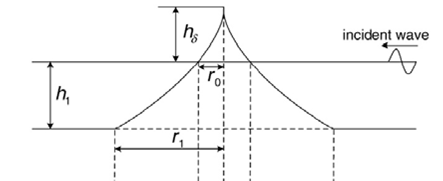
\includegraphics[width=0.4\textwidth]{img/VertSection.png}
 \caption{Vertical cross-section through circular island.}
 \label{t2d:shoal:fig:VertSection}
\end{figure}

This is a case where refraction and diffraction of a wave both occur.

\subsection{Numerical and physical parameters}
\telemac{2D} is run using the wave equation formulation and no
bed friction or viscosity.
Thompson boundary condition is used so waves could pass out from the modelled domain.
The implicitation coefficients are taken as 0.501 (the model is second order
accurate if implicitation = 0.5, but on the edge of instability as the scheme is
unstable if implicitation < 0.5) and the free surface gradient compatibility is
taken as 0.9 (recommended value).

\section{Results}
The model is compared with the analytical solution by contouring the wave
amplitude (Figure \ref{t2d:shoal:fig:ModelSol}) to compare with the analytical
solution (Figure \ref{t2d:shoal:fig:AnalSol}).
These figures are for a profile in which the depth varies as the 2/3 power of
the radius as shown in Figure \ref{t2d:shoal:fig:VertSection}.

\begin{figure}[!htbp]
 \centering
 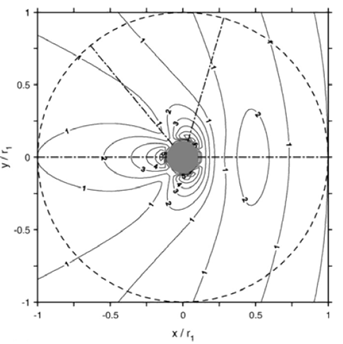
\includegraphics[width=0.4\textwidth]{img/AnalyticSolutionShoal.png}
 \caption{Wave amplitude contours for a circular island with $r_1 = 9r_0$, $r_0$ = 10~km, $h_1$ = 4~km. Analytical solution.}
 \label{t2d:shoal:fig:AnalSol}
\end{figure}

\begin{figure}[!htbp]
 \centering
 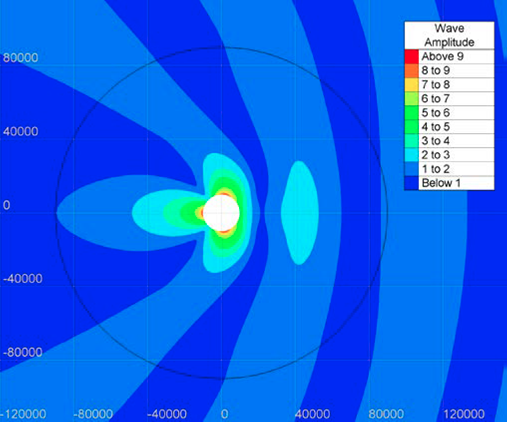
\includegraphics[width=0.4\textwidth]{img/ModelSolutionShoal.png}
 \caption{Wave amplitude contours for a circular island with $r_1 = 9r_0$, $r_0$ = 10~km, $h_1$ = 4~km. Model solution.}
 \label{t2d:shoal:fig:ModelSol}
\end{figure}

It can be seen that the wave height pattern is well reproduced for this situation.

Free surface elevation at the end of the simulation can be seen in Figures
\ref{fig:shoal:FreeSurface} and \ref{fig:shoal:FreeSurfaceZoom} (the latter is a
zoom around the circular island).

\begin{figure}[H]
 \centering
 \includegraphicsmaybe{[width=0.8\textwidth]}{../img/FreeSurface.png}
 \caption{Free surface elevation at final time.}
 \label{fig:shoal:FreeSurface}
\end{figure}

\begin{figure}[H]
 \centering
 \includegraphicsmaybe{[width=0.8\textwidth]}{../img/FreeSurfaceZoom.png}
 \caption{Free surface elevation at final time (zoom around the island).}
 \label{fig:shoal:FreeSurfaceZoom}
\end{figure}

%\section{Conclusion}
